\documentclass{article}

\usepackage{graphicx}

\newcommand{\Nif}{\rm $^{56}$Ni }

\begin{document}
\title{Plots for the $M_{ej}$ correlations}
\maketitle

%%##TO ADD TEXT
This document has the plots for the ejecta mass calculations using the measured NIR light curves of CSP-I objects. It also includes a short discussion of the distributions in the literature or from complementary methods.

\begin{itemize}

\item \Nif mass using Arnett's rule and $t_0$ using the Jeffrey 1999 formalism

\item \Nif mass from the nebular phase line and the ejecta mass from Scalzo et al 2014 relation (using the stretch values)

\item Calculated from Richard's MCMC 

\end{itemize}


\section*{Procedure}
In this section,  I describe the procedure used for calculating the $M_{Ni}$ and $M_{ej}$ values. I follow the steps in Stritzinger et al. 2006, but I have written down each part of the analysis so that it can be checked.

\begin{itemize}
\item I use an $R_V$ value for each SN (in this case 1.7) to calculate $A_V$ from the measured colour excess. 
\item The magnitudes are converted to dereddened fluxes and a bolometric light curve is calculated.  

\item $^{56}$Ni mass is calculated from the bolometric peak using Arnett's rule

\item $t_0$ is calculated by fitting a ${^56}$Co deposition function to the bolometric light curve between +40 and +100\,d

\item $M_{ej}$ is calculated as in Jeffrey 1999 using the same assumptions for $v_e$, $q$ and $\kappa_{\gamma}$ as in Stritzinger et al. 2006.
\end{itemize}

\subsection*{Nickel mass calculations}
For plots in this document, the Ni masses were calculated in the 'conventional' method, using multi-band data to construct a bolometric light curve. The sample of SNe for this calculation includes objects with significant (E(B-V) > .1) reddening. For these objects, the Ni masses calculated from the bolometric light curve will be sensitive to the $R_V$ value assumed. 

The objects with a high \Nif mass are  SN~2006et, SN~2007S, SN~2007le, SN~2008fp. These objects all have \textgreater 0.25 mag of extinction. Comparing the \Nif mass from the second maximum to the estimate from the peak suggests that the $R_V$=1.7 fit is significantly better than $R_V$ = 3.1. The measured $R_V$ values for these 4 SNe (from Burns et al. 2014 using maximum light photometry) is $\sim$ 1.7 which agrees well with the inference from the \Nif mass. This may also be further proof that 91T-like objects occur in dustier environments.


 %Using $R_V$ = 1.7 gives \Nif mass estimates com
 
\begin{figure}
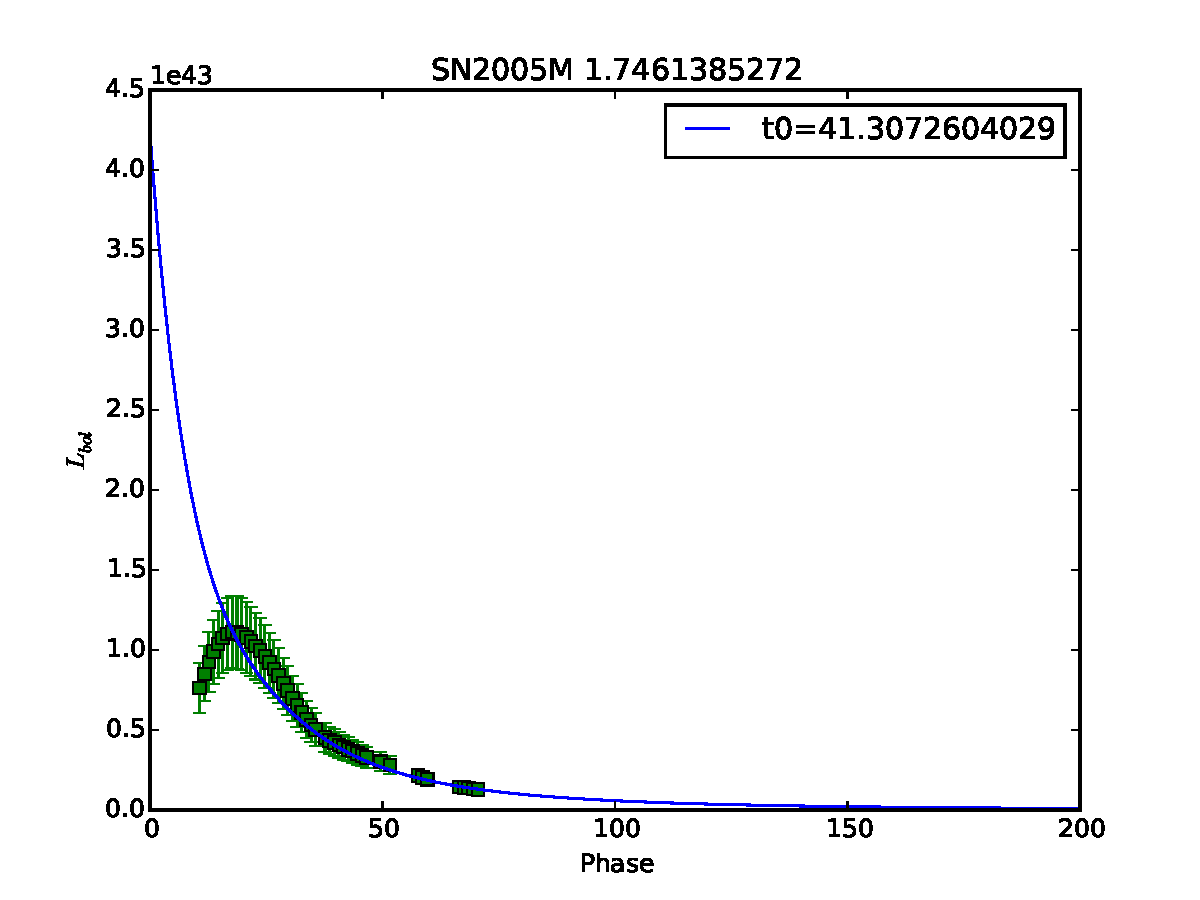
\includegraphics[width=.5\textwidth, trim = 0 0 30 30]{SN2005M.pdf}
\caption{Fitting the deposition curve to the bolometric light curve of SN~2005M}
\label{fig:fit}
\end{figure}

\begin{figure}
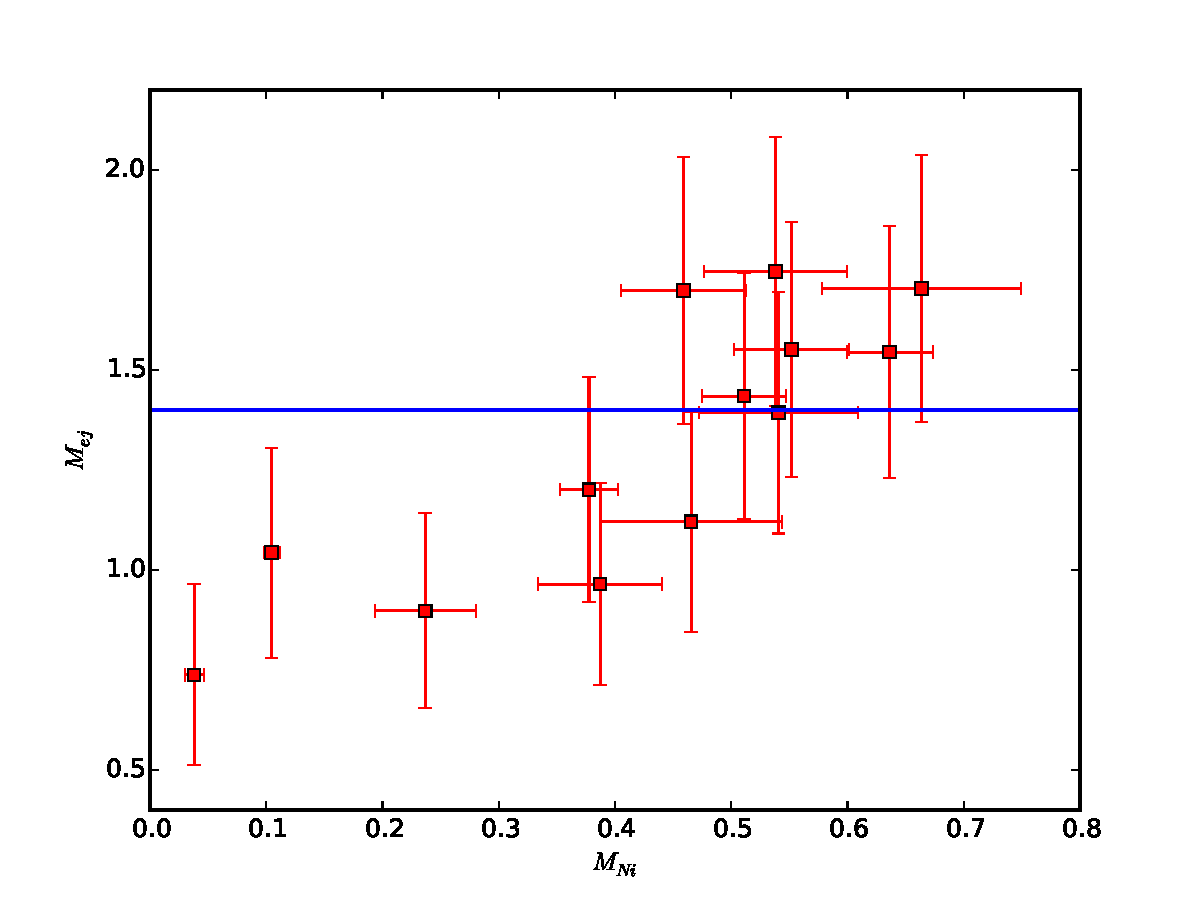
\includegraphics[width=.5\textwidth, trim = 0 0 30 30]{mej_mni_risetime.pdf}
\caption{Using a variable rise time for the Nickel mass calculations, the relation between M$_{ej}$- \Nif mass}
\label{fig:mej-mni}
\end{figure}

\begin{figure}
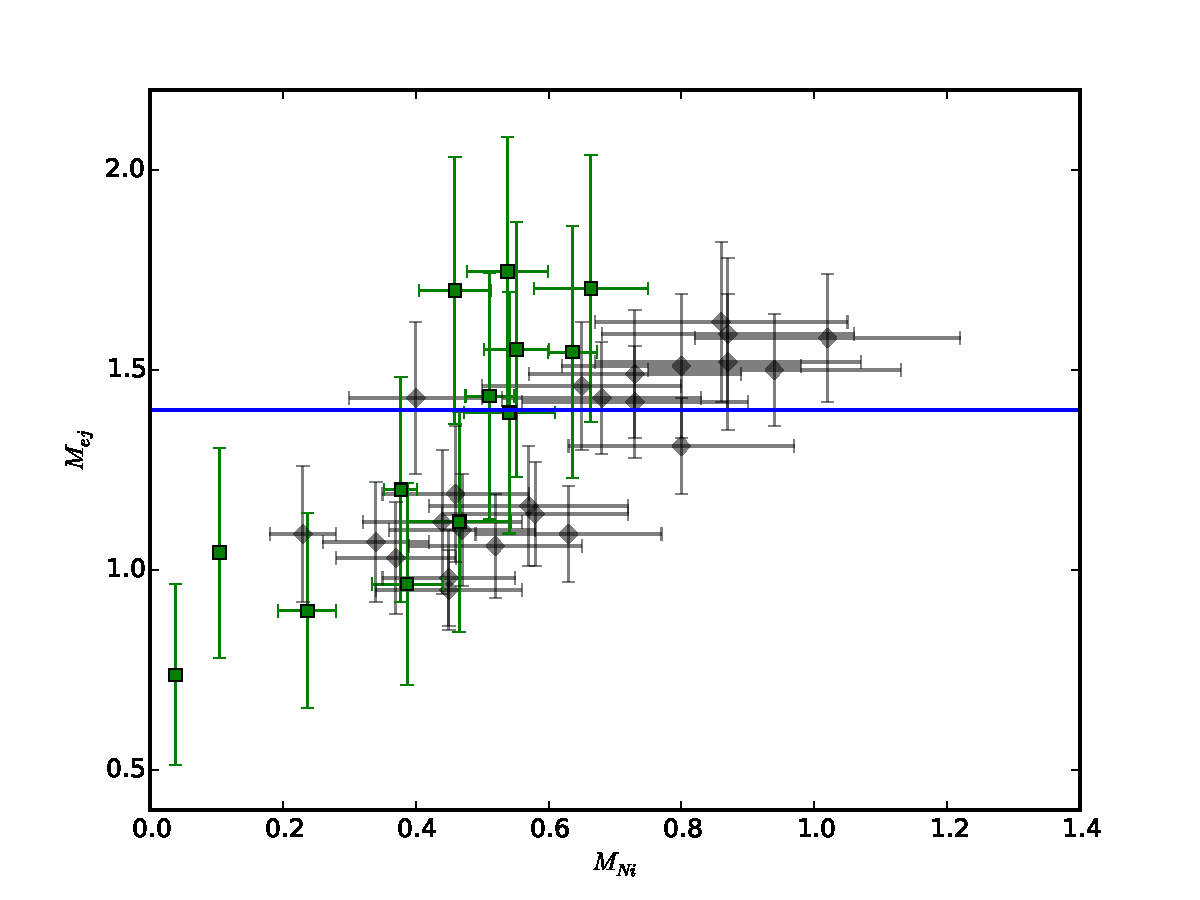
\includegraphics[width=.5\textwidth, trim = 0 0 30 30]{mej_mni_richard_comparison.pdf}
\caption{Comparing the SNe in Figure~\ref{fig:mej-mni} to the calculations by Richard}
\end{figure}

%Richard's sample doesn't include fast-decliners and uses the Bayesian framework.
\end{document}




